\chapter{Objective}
\section{Problem definition}

The problem addressed during the internship at the National Social Security Fund (CNAS) revolves around optimizing the efficiency and effectiveness of social security processes and services. CNAS serves a vast number of beneficiaries, and it is crucial to ensure that the delivery of social security benefits is streamlined, transparent, and accessible to all eligible individuals.

One of the primary challenges observed during the internship is the need to enhance the digital infrastructure and modernize the existing systems and processes at CNAS. This includes developing user-friendly web-based applications, improving data management and analysis, and implementing advanced technologies to automate and expedite various administrative and operational tasks.

Additionally, there is a growing demand for optimizing the coordination and collaboration between different departments within CNAS. Efficient communication, data sharing, and interdepartmental workflows are vital to ensure seamless service delivery and timely decision-making.

The problem definition also encompasses the need for continuous monitoring, evaluation, and improvement of social security programs and policies. CNAS must remain adaptive and responsive to evolving societal needs and challenges, while also ensuring fiscal sustainability and compliance with legal and regulatory frameworks.

Throughout the internship, efforts were focused on addressing these challenges and proposing practical solutions to enhance the overall performance of CNAS in delivering social security benefits and services. The problem definition served as a guiding framework for the assigned tasks and projects, fostering innovation, efficiency, and effectiveness in the operations of CNAS.

By identifying and addressing these challenges, CNAS can further strengthen its role as a leading institution in social security and provide enhanced support to beneficiaries, contributing to the social and economic development of [Country].
\newpage
\section{Introduction to CNAS Organization}
\subsection{Definition of CNAS organization}
The CNAS (Caisse Nationale des Assurances Sociales) is a public institution with specific management under Article 49 of Law No. 88-01 of January 12, 1988. It has legal personality and financial autonomy and is considered a merchant in its relations with third parties. The CNAS is responsible for managing social insurance benefits (illness, maternity, disability, and death), as well as occupational accidents and diseases (AO/D), and family allowances on behalf of the state. It also manages the collection, control, and litigation of contributions for financing benefits, as well as the management of the litigation related to the collection of subscriptions for financing rendered.

The CNAS assigns a national registration number to insured persons and employers and contributes to promoting the policy of prevention of AO/D and managing the AO/D prevention fund. It also manages benefits for beneficiaries of bilateral social security agreements, carries out medical control of beneficiaries, and undertakes actions to provide workers and their dependents with collective benefits in the form of health and social achievements. The CNAS also manages the aid and relief fund and concludes agreements with healthcare providers while ensuring the information of beneficiaries and employers.

The CNAS provides benefits to salaried workers, apprentices, job seekers, students, trainees in vocational training, disabled persons, veterans, social security beneficiaries (pensioners and annuitants), and beneficiaries of the lump sum solidarity allowance (sick, elderly and inactive persons). Dependents, including the spouse, minor children, unmarried inactive daughters, and dependent ascendants, are also eligible for benefits.

The CNAS covers healthcare and medication costs at 80\%, and in some cases 100\% (particularly for chronic diseases). Compensation for sick leave is 50\% of the salary for the first 15 days and is increased to 100\% of the salary beyond the 16th day, with a maximum duration of three years. Maternity benefits are fully covered, and working women are entitled to a 98-day maternity leave. The minimum amount of invalidity pensions is equal to 75\% of the guaranteed minimum wage. In the event of the insured person's death, a death benefit is paid to his or her dependents. Occupational risks are covered 100\% for healthcare and sick leave, and annuities are paid in the event of bodily harm or death resulting from occupational accidents or diseases.
\cite{cnas-presentation}
\newpage
\subsection{Organization of CNAS}
CNAS is managed by a Board of Directors and is under the supervision of the Minister of Labor, Employment and Social Security. Its headquarters is located in Algiers (BEN AKNOUN), and it has national jurisdiction with both central and local services.\footnote{CNAS. (n.d.). Presentation of CNAS. Retrieved from \url{https://www.cnas.dz/}.}

\medskip To fulfill its missions, CNAS has: 
\begin{table}[htbp]
  \centering
  \begin{tabular}{|p{10cm}|l|}
  \hline
  \textbf{Structure} & \textbf{Number} \\
  \hline
  General Directorate & 1 \\
  \hline
  Provincial agencies(including 2 in Algiers)  & 49 \\
  \hline
  Payment structures & 826 \\
  \hline
  Payment centers & 356 \\
  \hline
  Payment branches & 401 \\
  \hline
  Local correspondences & 69 \\
  \hline
  Specialized clinics (pediatric heart surgery, orthopedics and rehabilitation, ENT, dental) & 4 \\
  \hline
  Regionval centers for medical imaging & 4 \\
  \hline
  Diagnostic and treatment centers & 35 \\
  \hline
  Pharmaceutical offices & 55 \\
  \hline
  Nurseries and kindergartens & 30 \\
  \hline
  Printing house in Constantine & 1 \\
  \hline
  Family social center in Ben Aknoun & 1 \\
  \hline
  \end{tabular}
  \caption{CNAS Structures}
  \end{table}

\newpage
\subsection{CNAS Organigram}
the CNAS organigram is made up of various departments, subdivisions, and services that work together to manage CNAS operations and deliver services to its beneficiaries.

\medskip 

Here is the CNAS organigram : 
\begin{figure}[h]
  \centering
  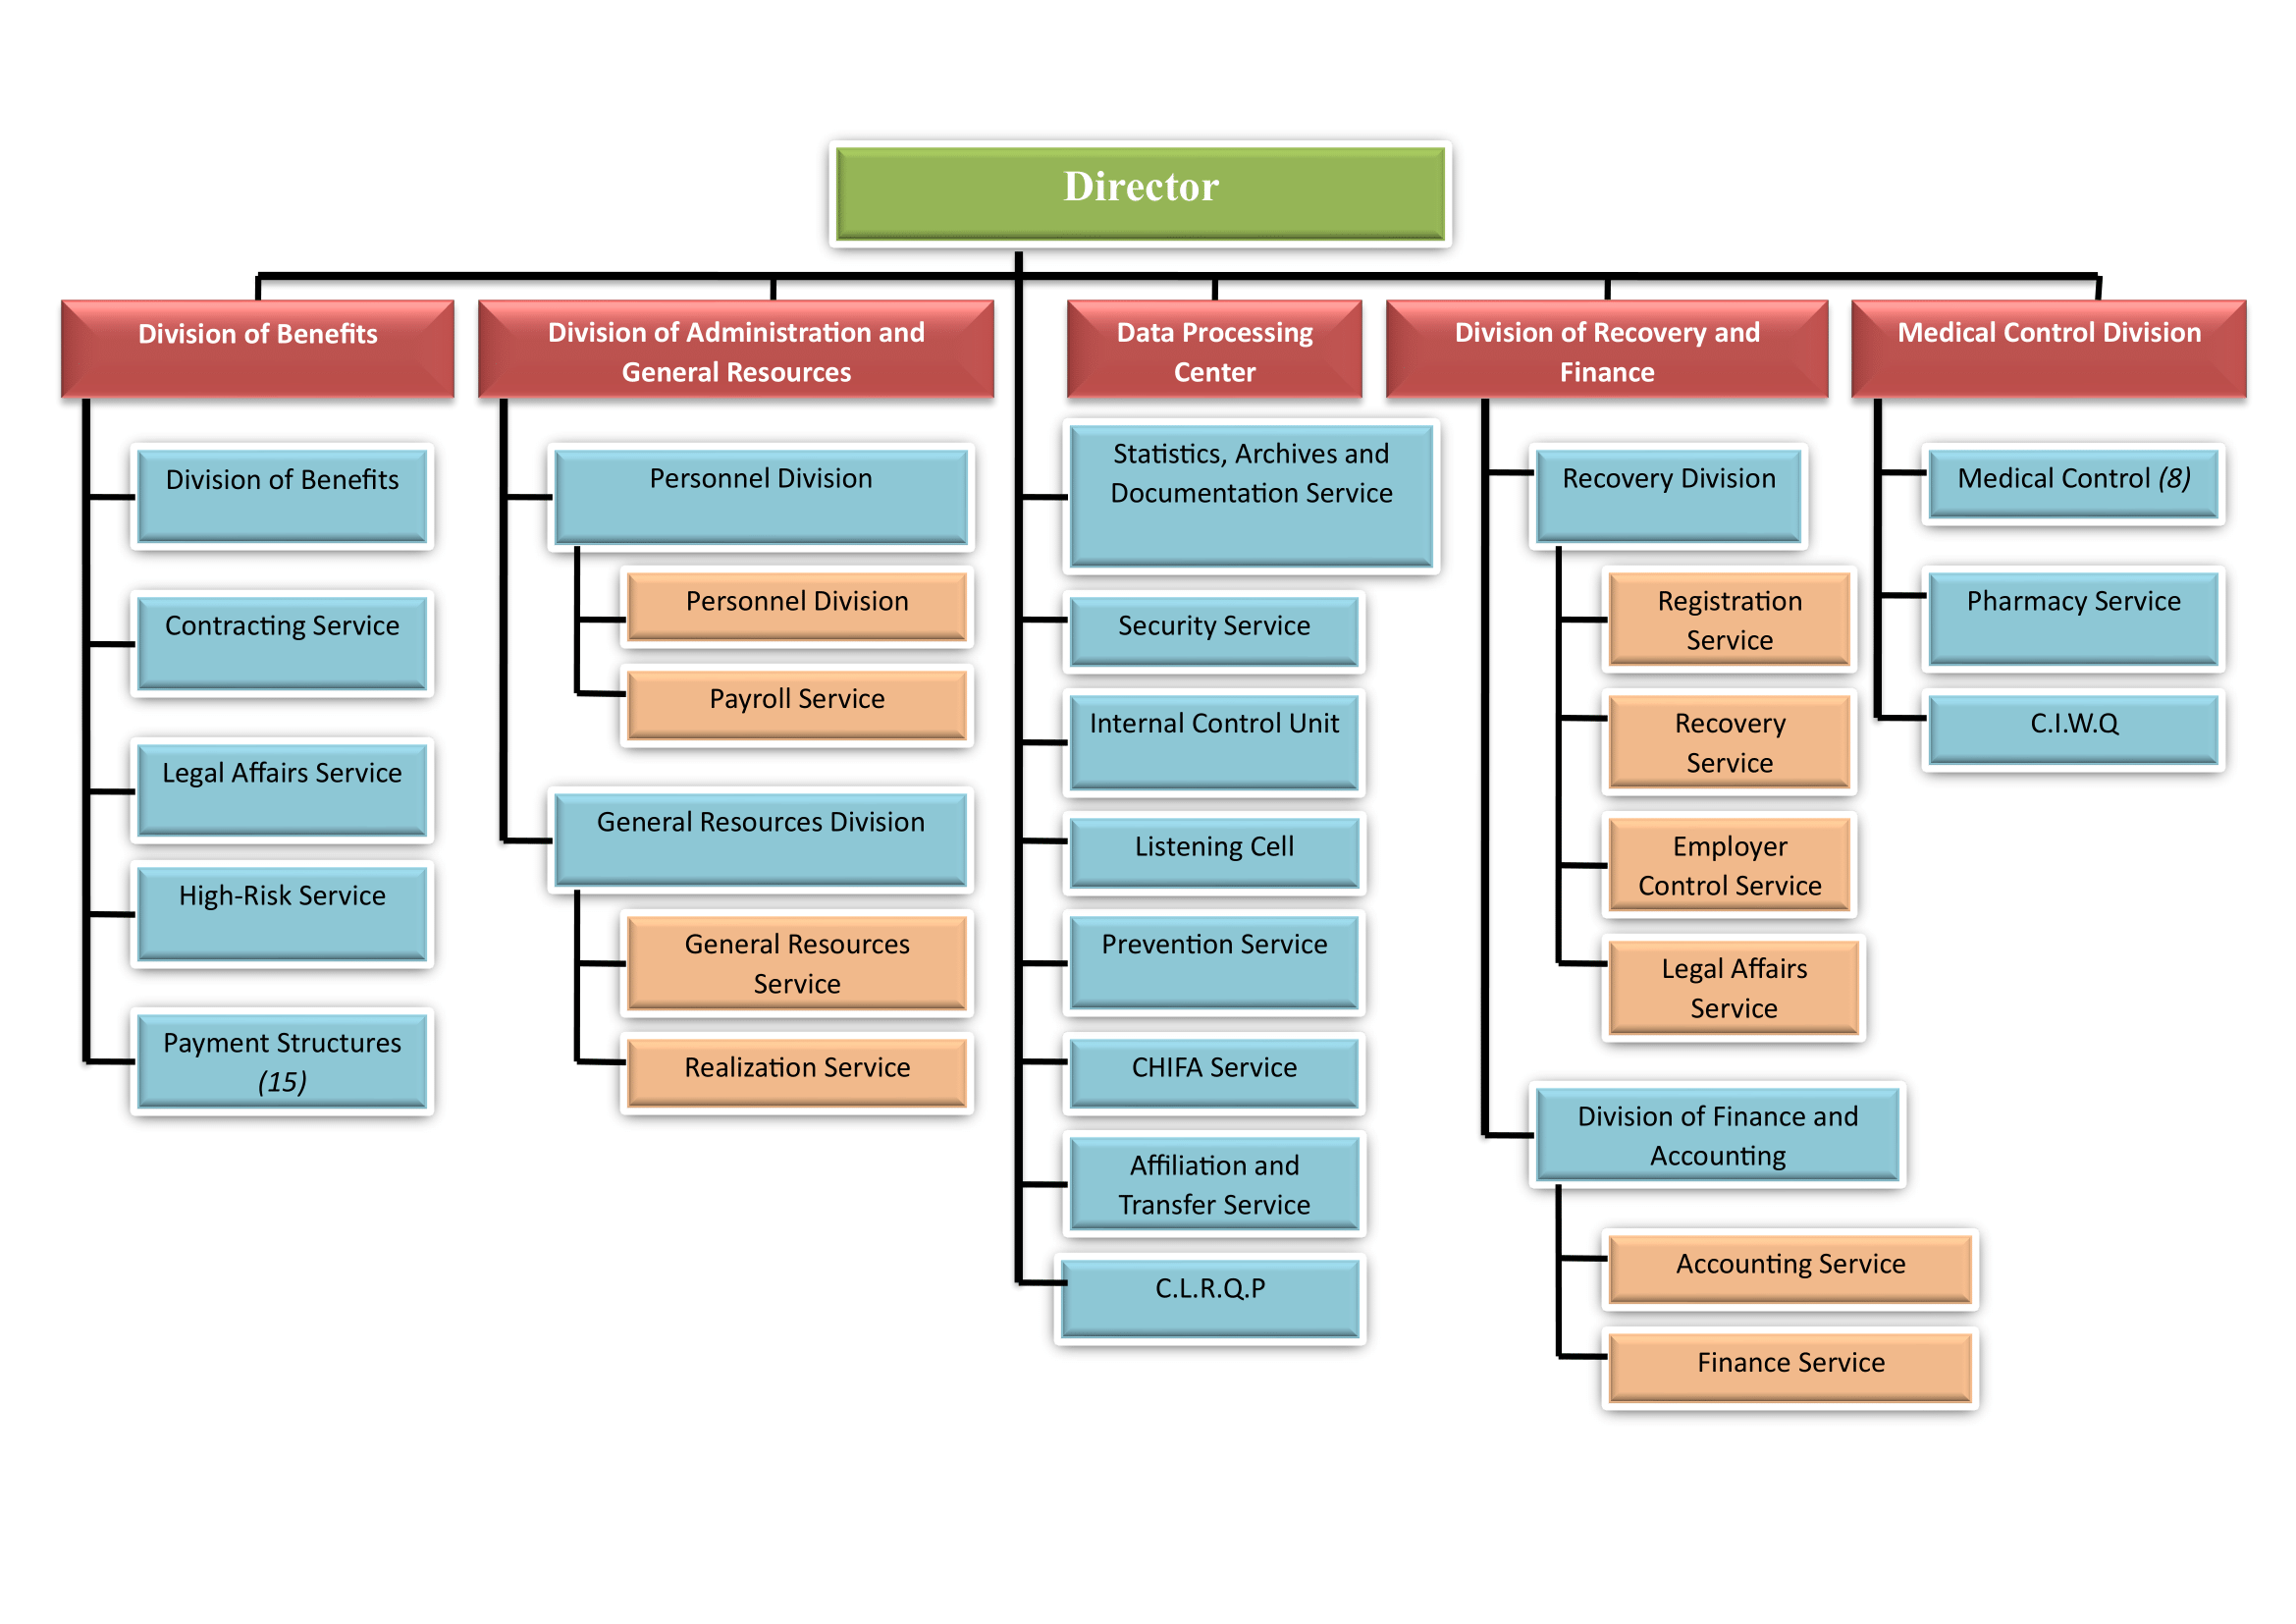
\includegraphics[width=1.0\textwidth]{organigram.png}
  \caption{Organigram of CNAS}
  \label{fig:organigram}
\end{figure}
\subsection{CNAS Services}
CNAS provides a range of services related to social security and healthcare to the Algerian population. These services include:
\begin{itemize}
    \item \textbf{Healthcare services:} CNAS operates its own specialized clinics and medical facilities, including four specialized clinics for cardiac surgery, orthopedics and rehabilitation, otorhinolaryngology, and dental care. It also runs 35 diagnostic and treatment centers, 55 pharmacies, and four regional medical imaging centers.

    \item \textbf{Social security services:} CNAS provides social security services to its members and their families, including health insurance, maternity leave benefits, disability benefits, and retirement pensions. It also offers services related to workplace safety and injury compensation.

    \item \textbf{Family services:} CNAS operates 30 nurseries and childcare centers to support working parents.

    \item \textbf{Payment services:} CNAS manages a network of payment centers and local correspondents to ensure the timely payment of social security benefits to its members.
\end{itemize}
\subsection{  Importance of CNAS services for the Algerian society}
These services are essential for the Algerian society, as they help provide access to healthcare and social security benefits to millions of people. CNAS's role in ensuring workplace safety and providing compensation for work-related injuries is also crucial in protecting the rights and wellbeing of workers across Algeria.

